%	Prova essay
\documentclass[a4paper, 12pt]{article}

\usepackage[protrusion=true,expansion=true]{microtype} % Better typography
\usepackage{graphicx} 
\usepackage{subfig}
\usepackage{wrapfig} %in-line image

\usepackage[dvipsnames]{xcolor}
\usepackage{listings}
%\usepackage{alloy-style}

\usepackage[T1]{fontenc}

\usepackage[hyphens]{url}
\usepackage{quoting}
\usepackage{pdfpages}
%\usepackage[unicode,pdftex,plainpages=false,linktoc=all, hyperindex,citecolor=green,urlcolor=blue ]{hyperref}
\quotingsetup{font=small}

\usepackage[printonlyused]{acronym}

\usepackage{mathtools}
\usepackage{algorithm}
\usepackage{setspace}
\usepackage[noend]{algpseudocode} %noend removes the "end" 

\makeatletter
\newcommand{\myparagraph}[1]{\paragraph{#1}\mbox{}\\}
\renewcommand\@biblabel[1]{\textbf{#1.}} % Change the square brackets for each bibliography item from '[1]' to '1.'
\renewcommand{\@listI}{\itemsep=0pt} % Reduce the space between items in the itemize and enumerate environments and the bibliography

% \renewcommand{\abstractname}{\large Introduction} %%Renaming the abstract

%-----title at right corner---------------------------------------
\renewcommand{\maketitle}{ 
\begin{figure}[h]
\centering

\includegraphics[width=7cm]{Images/LogoPolimi}\\[.5cm]
\end{figure}

\vspace{50pt}

\begin{flushright} % Right align
\@date 

{\huge\@title} % Increase the font size of the title
\vspace{140pt} % Some vertical space between the title and author name


\begin{tabular}{ l l c}
\large Blanco &  \large Federica & \large 875487\\
\large Casasopra & \large Fabiola & \large 864412\\
\end{tabular}

\vspace{40pt} % Some vertical space between the author block and abstract
\end{flushright}
\centering
\textsl{\large Software Engineering 2 Project}\\
2016/2017
}

%\title{\textbf{Unnecessarily Long Essay Title}\\ % Title
%Focused and Deliciously Witty Subtitle} % Subtitle
\title{\textbf{PowerEnJoy}\\[3mm]
Integration Test Plan Document}

\author{Blanco Federica\\Casasopra Fabiola%\textsc{Nomi} % Author -> fix with more names
} 

\date{15 January 2017} % Date

%----------------------------------------------------------------------------------------

\begin{document}

\begin{titlepage}

\thispagestyle{empty}
\maketitle % Print the title section

\end{titlepage}


%\input{Acronym.tex}
%\renewcommand{\abstractname}{Summary} % Uncomment to change the name of the abstract to something else
%\vspace{30pt} % Some vertical space between the abstract and first section
\thispagestyle{empty}
\tableofcontents
\clearpage 
\thispagestyle{empty}
\listoffigures
\clearpage 
%\listoftables
%\clearpage 

%\pagenumbering{roman}
%\input{Sections/Abstract.tex} %optional
\newpage
\pagenumbering{arabic}
\section{Introduction} \label{sec:intro}
In this chapter there are the main purpose of this document, the project's scope and its actors and goals, some definitions who help to understand the content of the document and some reference documents that are used to make this one. 

\subsection{Purpose} \label{subsec:purpose}
This document is called \emph{\acl{rasd}}, also knowed as the acronym \acs{rasd}. Its purpose is to communicate to customers what is understanding about functional and not-functional requirements based, the limitations and obstacles for implement this system, the constraints founded and for modeling the customer's need. This document is also addressed to developers and programmers who have to implements all the requirements then it must be more complete and correct than possible. It is a contract with customers therefore it must show use cases to allow everyone to understand what the system will do and in what domain it can be used. Project manager can use this document to make an evaluation of costs and size of the project.


\subsection{Scope} \label{subsec:scope}
The aim of the project called PowerEnJoy is to provide a car-sharing service that involves only electric cars. All people who wants to share a car must be able to register at the system using credentials such as name, surname, e-mail, nickname and giving a valid information payment (number of credit card) that is needed to pay for the service. When the user receive the password to log in, he can find available cars in a specific location and, if he wants, he can reserve it. The system unlocks the car as soon as the user is nearby and keep informed of the amount of the service with a screen on the car; when the car is in one of the safe areas, indicated in a list that can be consulted on-line, the system locks it after the person exit from it. The project has also the purpose to encouraged people to left at home their pollutants cars and takes with other people the electric car: in fact if there are at least two passengers with the driver he has a 10 per cent discount on the ride. If the user leaves the car in the safe area with more than half of the battery he has a 20 per cent discount on the ride and if he recharged the car he will have 30 per cent discount. But if the user leaves the car far away from a safe area or with more than 80 per cent of empty battery, the system charges 30 per cent more on the ride.

%Identifies the product and application domain
%Analysis of the world and of the shared phenomena
\subsection{Domain Properties} \label{subsec:domain}
We supposed that our domain has this properties:
\begin{itemize}
\item[\textbf{D1}]The nickname and the e-mail are unique to identify an user.
\item[\textbf{D2}]The e-mail must be syntactically correct and must correspond to an existing server.
\item[\textbf{D3}]The car's position can be knowed thanks to GPS.
\item[\textbf{D4}]The charge is calculated considering time passed using the car, given a specific fee per minute.
\item[\textbf{D5}]In the car there is a sensor that idicates how many people there are in the car and another sensor which indicates the battery level.
\item[\textbf{D6}]For each car there is an insurance.
\item[\textbf{D7}]Reservation's time must be included between 00:00 and 23:59.
\item[\textbf{D8}]The position inserted by the user must be an existing place.
\end{itemize}


\subsection{Actors} \label{subsec:actors}
Here there are a list of the actors who can operate with the system.
\begin{itemize}
\item[\textbf{->}] VISITOR: the person who visits the systems but that is not log-in in the site, he can only see the home page and the page with the form for the registration, where he must provide all the requested information. Moreover, he has the possibility to log-in with the password given by the system when the registration is successfully committed. 
\item[\textbf{->}] USER: the person who has successfully log-in. He can do all the operations provided by the system through the user interface such as reserve a car or consult the list of available cars or say to the system that he is nearby the reserved car. 
\end{itemize}

\subsection{Goals} \label{subsec:goals}
In this section we want to explain exhaustively what are our system's goal.
\begin{itemize}
\item[\textbf{G1}] The system must be able to allow visitor to register.
\item[\textbf{G2}] The system must be able to give a password to a visitor successfully registered.
\item[\textbf{G3}] The system must be able to allow visitor to log in.
\item[\textbf{G4}] The system must be able to provide to the user the list of available cars near his position or a specific location.
\item[\textbf{G5}] The system must be able to allow user to reserve a car up to one hour before it is picked up.
\item[\textbf{G6}] If the user is near his reserved car the system must unlock it.
\item[\textbf{G7}] The system must be able to charge the user.
\item[\textbf{G8}] The system must be able to keep informed the user about the charge trough a display in the car.
\item[\textbf{G9}] If the user not pick up the car after one hour from the registration, the system must be able to delete the registration giving a fee of 1 euro to the user.
\item[\textbf{G10}] The system must allow user to delete a reservation before one hour is passed.
\item[\textbf{G11}] If a registration is deleted the system must be able to make the car available.
\item[\textbf{G12}] The system must lock a car when it is left in a safe area.
\item[\textbf{G13}] The system must be able to apply discount if is verified one case.
\item[\textbf{G14}] The system must be able to apply an increase to the amount of a ride if is verified a specific case.


\end{itemize}


\subsection{Definitions, acronyms, abbreviations} \label{subsec:def-ac-ab}

\subsubsection{Definitions} \label{def}
This section is necessary for avoid ambiguity or misunderstanding during the reading of this document. 
\begin{itemize}
\item VISITOR: he is a person that is not register in the system, he can only see the homepage and go to the form for the registration.
\item USER: he is a person that is registered in the system; he is identified by a name, surname, nickname, e-mail, password (given by the system at the end of the registration), telephone number, address and all the payment information such as number of credit card and card's deadline that must be verified by the system. He can do all the services that are provided by "\emph{PowerEnJoy}".
\item CAR: we intend an electric car that can be shared trough the system. It can be available or reserved and the system will lock and unlock it when is necessary. It is parked in a safe area.
\item RIDE: with this term we intend all the route that a user accomplishes with the same car from the moment when he pick up the car to the moment when I left it in a safe area.   
\item CHARGE: we intend the debt that the user must pay at the end of a ride; it is calculate from a specific amount of money per minute which start from the begin of the ride to the end of it. That can be also modified  by some discount, if is verified a particular situation, or a fee. It exists also a charge if the user reserve a car but he don't pick it up after one hour from the reservation.  

\end{itemize}

\subsubsection{Acronyms} \label{acr}
Here there is the acronims list:

%------------Acronyms----------
\begin{acronym}[RASD] %put here the first acronym

\acro{rasd}[RASD]{Requirements Analysis and Specifications Document}
\acro{uml}[UML]{Unified Modeling Language}
\acro{api}[API]{Application Programming Interface}
\acro{db}[DB]{DataBase}
\acro{os}[OS]{Operating System}
%lists of used acronyms

\end{acronym}

\subsubsection{Abbreviations} \label{abbre}
\begin{itemize}
\item \textbf{Gn} : indicates the goal's number
\item \textbf{Rn} : indicates the requirement's number for a specific goal
\item \textbf{Dn} : indicates the domain's number
\end{itemize}


\subsection{Overview} \label{subsec:overview}
This document is structured in four parts:
\begin{itemize}
\item[\textbf{Part 1}]In the first part there is an introduction with this document's purpose, the scope of this project and its aim, the actor that can use  the system and in which way, some definitions to avoid misunderstanding during the reading of the document and, most important, the goal of our project described all in brief but comprehensive way.  
\item[\textbf{Part 2}]In the second part there are more specifications about the requirements, the interfaces with external agents, constraints and assumptions.
\item[\textbf{Part 3}]The third part is very important because there are all the models for the requirement: they are modeled using \acs{uml} diagrams such as \emph{Use Case} and \emph{Sequence Diagram} and using Alloy. They are very important to understand all the functionality of the system.  
\item[\textbf{Part 4}]In this part there is the Appendix with other informations and the hour spent by all of us to make this document.
\end{itemize}
%Describes contents and structure of the remainder of the RASD

\subsection{Reference Documents} \label{ref-doc}

\begin{itemize}
\item[\textbf{--}] Specification document: Assignments AA 2016-2017.pdf
\item[\textbf{--}] Standard for \acs{rasd}: IEEE Std 29148-2011
\item[\textbf{--}] \acs{api} information: 
\url{https://developers.google.com/maps/}

\url{documentation/geolocation/intro}

\end{itemize}




\newpage
\section{Integration Strategy} \label{sec:intstra}

\subsection{Entry Criteria}
%Specify the criteria that must be met before integration testing of specific elements may begin (e.g., functions must have been unit tested).

In this part of the document, we are going to specify the criteria that must be met before integration testing of specific elements may begin:

\begin{itemize}

\item[\textbf{--}] The \acl{rasd} and the \acl{dd} must be already completed, in order to know the interaction of the various components and their expected behaviour;

\item[\textbf{--}] Each component of our software must have successfully passed the Unit Testing;

\item[\textbf{--}] So, the correct version of our application is moved into the integration testing environment;

\item[\textbf{--}] All the code of our project must be already written and so the major functionality must be present;

\item[\textbf{--}] Our project should satisfy the memory requirements specified in the \acs{rasd};

\item[\textbf{--}] The database should be ready and its tables should already be populated with the initial data.

\end{itemize}

\subsection{Elements to be Integrated}
%Identify the components to be integrated,refer to your design document to identify such components in a way that is consistent with your design.

As we have shown in the \acl{dd} related to our project PowerEnJoy, the system relies on many high-level components, each one implementing a specific set of functionalities, that interacts between them.
Since we have decided to follow a modular approach, each component is the result of the combination of various subcomponents.
However, since we haven't fully defined all low-level component needed for our system, we think it is better to focus our integration testing only on the Business Logic and its components (for further information, see \textit{Section 2} of the \acl{dd}). By doing this choice, we have to consider that, in the following evolution of our project, the needed subcomponents will be created and further \acl{it} must be carried out.
 
So, for what we said above, the elements to be integrated are the following:

\begin{itemize}

\item[\textbf{--}] Web Component and Business Logic Component, testing the  direct connections between Managed Beans and their corresponding Managers;

\item[\textbf{--}] the subcomponents of the Business Logic Component, integrating them, each one with the needed others.

\end{itemize}

\subsection{Integration Testing Strategy}
%Describe the integration testing approach(top-­‐down, bottom-­‐up, functional groupings,etc.) and the rationale for the choosing that approach.
As we explained above, in this stage of the development we haven't fully defined the hierarchy of all subcomponents and subsystem.
For this reason, we will have an \acl{it} strategy for a single abstract layer and we have to keep in mind that other lower level subcomponents will be implemented.
Although it is not possible to define the final integration test strategy, we think that, as far as we know at this stage, the better strategy we can apply is the top-down approach.
Moreover, the choice of this strategy allows us to test the new subcomponent following the downward development.

\subsection{Sequence of Component/Function Integration}
%NOTE: The structure of this section may vary depending on the integration strategy you select in Section 2.3; use the structure proposed below as a non mandatory guide

\vspace{40pt}

\begin{figure}[htbp]
\centering
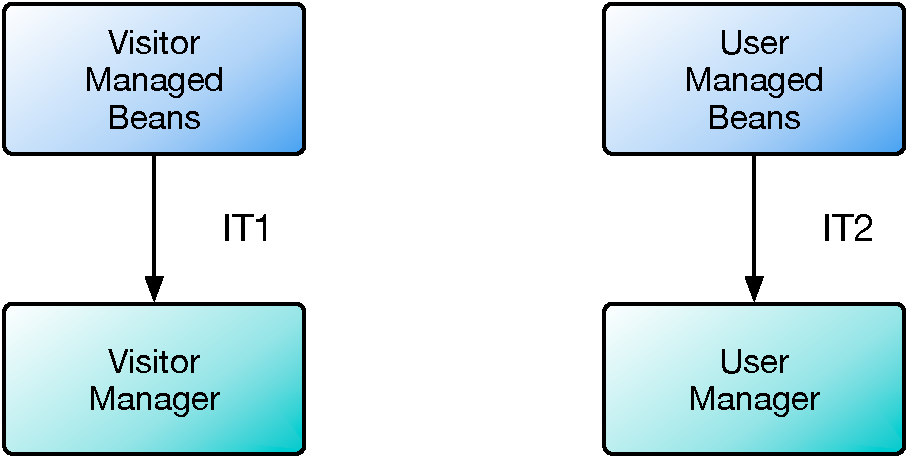
\includegraphics[width=0.6\textwidth]{Images/IT1-2.pdf}
\vspace{16pt}
\caption{Managed Beans and corresponding Managers connections}
\label{fig:it1-2}
\end{figure}

\vspace{16pt}

\begin{table}[htbp]
\begin{center}
\begin{tabular}[t]{cccc}

\hline
\textbf{ID} & \textbf{Components} & \textbf{\acs{it}} & \textbf{\acs{tp}}\\
\hline
IT1 & \enspace Visitor Managed Beans $\rightarrow$ Visitor Manager \enspace & \ref{sssec:IT1} & \ref{sssec:TP1}\\
\hline
IT2 & \enspace User Managed Beans $\rightarrow$ User Manager \enspace & \ref{sssec:IT2} & 
\ref{sssec:TP1}\\
\hline

\end{tabular}
\caption{Managed Beans and corresponding Managers connections}
\end{center}
\end{table}

\clearpage

\vspace{120pt}
\begin{figure}[htbp]
\centering
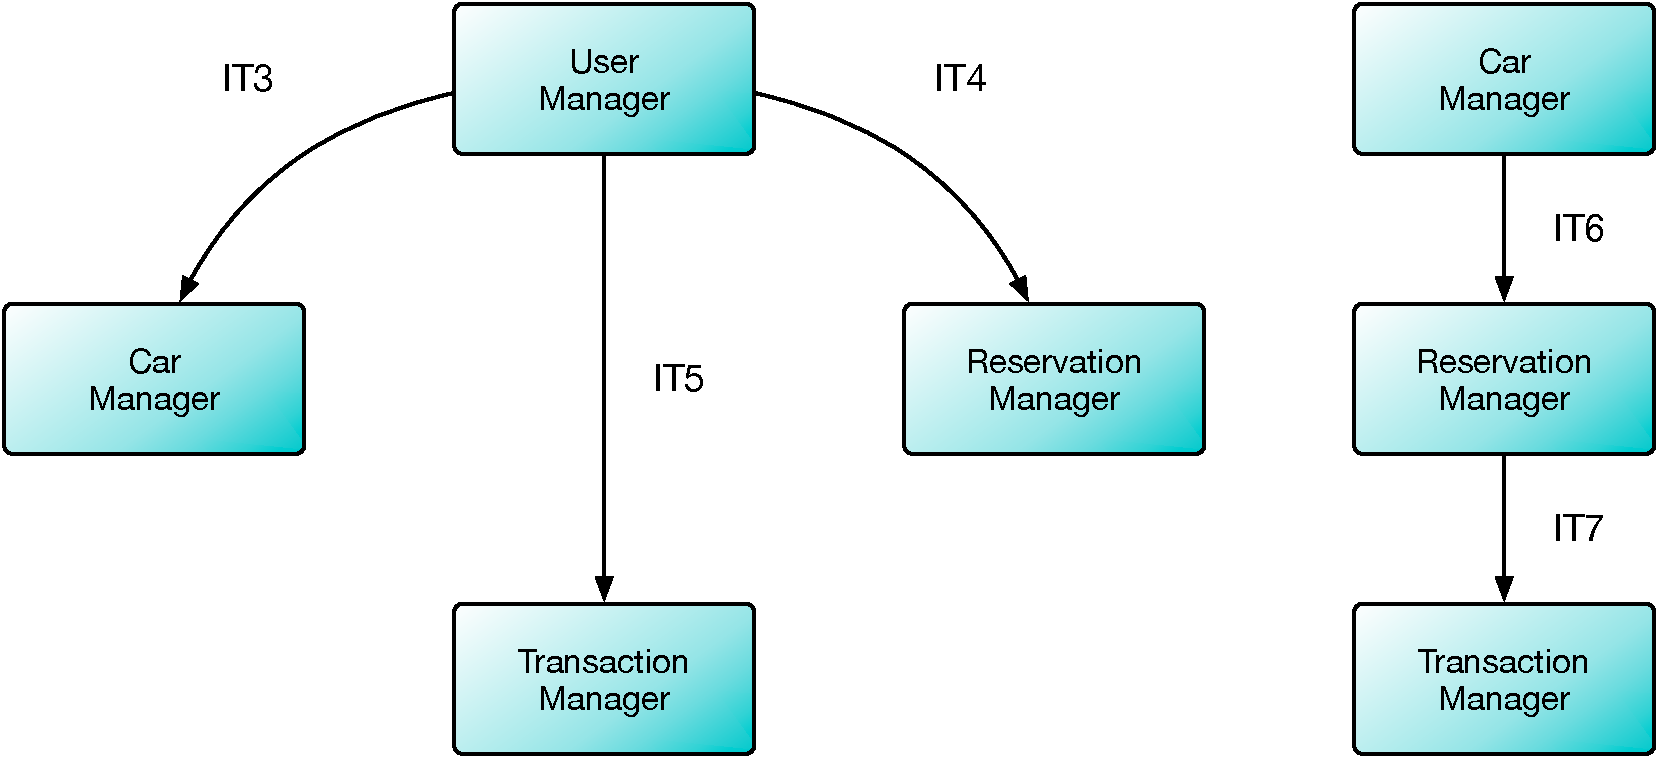
\includegraphics[width=\textwidth]{Images/IT3-7.pdf}
\vspace{16pt}
\caption{Business-tier subcomponents connections}
\label{fig:it3-7}
\end{figure}

\vspace{16pt}

\begin{table}[htbp]
\begin{center}
\begin{tabular}[t]{cccc}

\hline
\textbf{ID} & \textbf{Components} & \textbf{\acs{it}} & \textbf{\acs{tp}}\\
\hline
IT3 & \enspace User Manager $\rightarrow$ Car Manager \enspace & \ref{sssec:IT3} & \ref{sssec:TP2}\\
\hline
IT4 & \enspace User Manager $\rightarrow$ Reservation Manager \enspace & \ref{sssec:IT4} & \ref{sssec:TP2}\\
\hline
IT5 & \enspace User Manager $\rightarrow$ Transaction Manager \enspace & \ref{sssec:IT5} & \ref{sssec:TP2}\\
\hline
IT6 & \enspace Car Manager $\rightarrow$ Reservation Manager \enspace & \ref{sssec:IT6} & \ref{sssec:TP2}\\
\hline
IT7 & \enspace Reservation Manager $\rightarrow$ Transaction Manager \enspace & \ref{sssec:IT7} & \ref{sssec:TP2}\\
\hline


\end{tabular}
\caption{Business-tier subcomponents connections}
\end{center}
\end{table}

\clearpage

\begin{figure}[htbp]
\centering
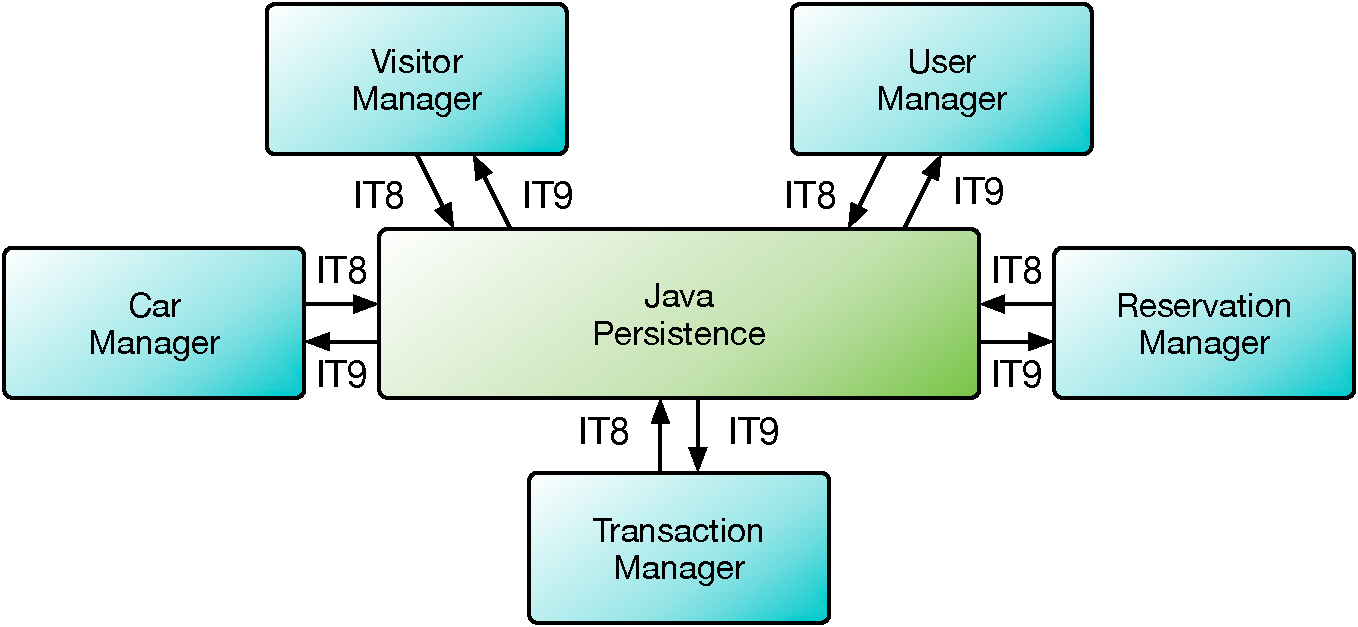
\includegraphics[width=0.9\textwidth]{Images/IT8-9-.pdf}
\vspace{16pt}
\caption{Business-tier subcomponents and Java Perstistence connections}
\label{fig:it8-9}
\end{figure}

\begin{table}[htbp]
\begin{center}
\begin{tabular}[t]{cccc}

\hline
\textbf{ID} & \textbf{Components} & \textbf{\acs{it}} & \textbf{\acs{tp}}\\
\hline
IT8 & \enspace User Manager $\rightarrow$ Java Persistence \enspace & \ref{sssec:IT8} & \ref{sssec:TP3}\\
\hline
IT8 & \enspace Visitor Manager $\rightarrow$ Java Persistence \enspace & \ref{sssec:IT8} & \ref{sssec:TP3}\\
\hline
IT8 & \enspace Car Manager $\rightarrow$ Java Persistence \enspace & \ref{sssec:IT8} & \ref{sssec:TP3}\\
\hline
IT8 & \enspace Reservation Manager $\rightarrow$ Java Persistence \enspace & \ref{sssec:IT8} & \ref{sssec:TP3}\\
\hline
IT8 & \enspace Transaction Manager $\rightarrow$ Java Persistence \enspace & \ref{sssec:IT8} & \ref{sssec:TP3}\\
\hline
IT9 & \enspace Java Persistence $\rightarrow$ User Manager \enspace & \ref{sssec:IT9} & \ref{sssec:TP3}\\
\hline
IT9 & \enspace Java Persistence $\rightarrow$ Visitor Manager \enspace & \ref{sssec:IT9} & \ref{sssec:TP3}\\
\hline
IT9 & \enspace Java Persistence $\rightarrow$ Car Manager \enspace & \ref{sssec:IT9} & \ref{sssec:TP3}\\
\hline
IT9 & \enspace Java Persistence $\rightarrow$ Reservation Manager \enspace & \ref{sssec:IT9} & \ref{sssec:TP3}\\
\hline
IT9 & \enspace Java Persistence $\rightarrow$ Transaction Manager \enspace & \ref{sssec:IT9} & \ref{sssec:TP3}\\
\hline

\end{tabular}
\caption{Business-tier subcomponents and Java Perstistence connections}
\end{center}
\end{table}

\clearpage

\vspace{120pt}
\begin{figure}[htbp]
\centering
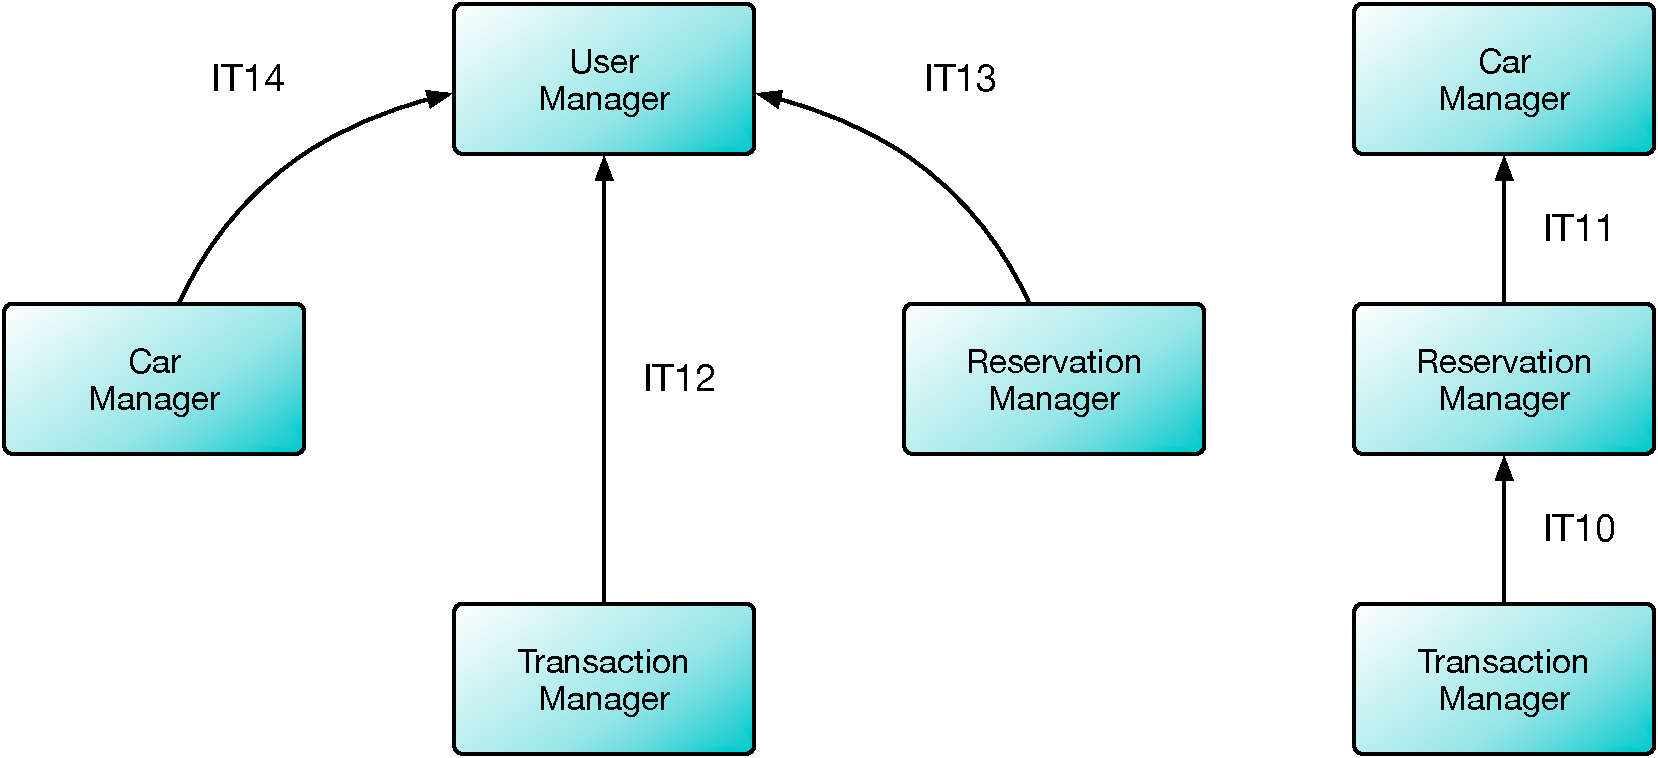
\includegraphics[width=\textwidth]{Images/IT10-14.pdf}
\vspace{16pt}

\label{fig:it10-14}
\caption{Business-tier subcomponents connections}
\end{figure}
\vspace{16pt}

\begin{table}[htbp]
\begin{center}
\begin{tabular}[t]{cccc}

\hline
\textbf{ID} & \textbf{Components} & \textbf{\acs{it}} & \textbf{\acs{tp}}\\
\hline
IT10 & \enspace Transaction Manager $\rightarrow$ Reservation Manager \enspace & \ref{sssec:IT10} & \ref{sssec:TP4}\\
\hline
IT11 & \enspace Reservation Manager $\rightarrow$ Car Manager \enspace & \ref{sssec:IT11} & \ref{sssec:TP4}\\
\hline
IT12 & \enspace Transaction Manager $\rightarrow$ User Manager \enspace & \ref{sssec:IT12} & \ref{sssec:TP4}\\
\hline
IT13 & \enspace Reservation Manager $\rightarrow$ User Manager \enspace & \ref{sssec:IT13} & \ref{sssec:TP4}\\
\hline
IT14 & \enspace Car Manager $\rightarrow$ User Manager \enspace & \ref{sssec:IT14} & \ref{sssec:TP4}\\
\hline

\end{tabular}
\caption{Business-tier subcomponents connections}
\end{center}
\end{table}

\clearpage

\vspace{120pt}

\begin{figure}[htbp]
\centering
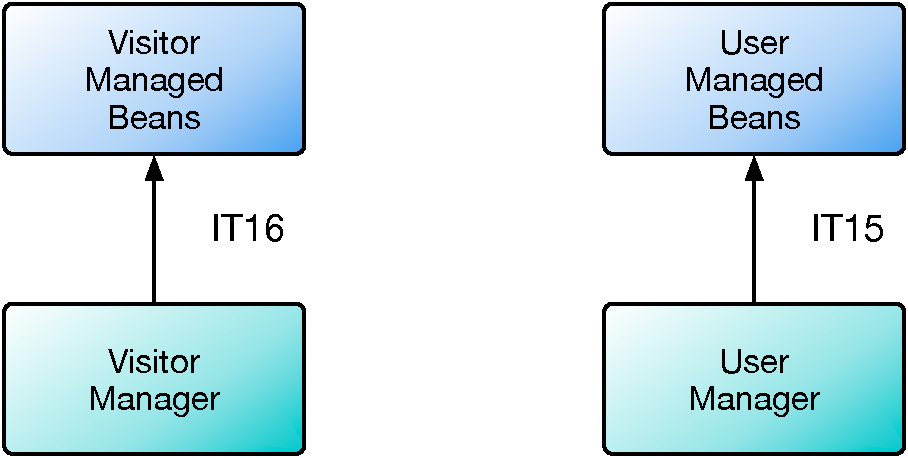
\includegraphics[width=0.6\textwidth]{Images/IT15-16.pdf}
\vspace{16pt}
\caption{Managed Beans and corresponding Managers connections}
\label{fig:it15-16}
\end{figure}

\vspace{16pt}

\begin{table}[htbp]
\begin{center}
\begin{tabular}[t]{cccc}

\hline
\textbf{ID} & \textbf{Components} & \textbf{\acs{it}} & \textbf{\acs{tp}}\\
\hline
IT15 & \enspace User  Manager$\rightarrow$ User Managed Beans \enspace & \ref{sssec:IT15} & \ref{sssec:TP5}\\
\hline
IT16 & \enspace Visitor Manager $\rightarrow$ Visitor Managed Beans \enspace & \ref{sssec:IT16} & \ref{sssec:TP5}\\
\hline

\end{tabular}
\caption{Managed Beans and corresponding Managers connections}
\end{center}
\end{table}

\clearpage
\newpage
\section{Individual Steps and Test Description} \label{sec:istd}
%For each step of the integration process above, describe the type of tests that will be used to verify that the elements integrated in this step perform as expected. Describe in general the expected results of the test set. You may refer to Chapter 3 and Chapter 4 of the test plan example[1] as an example of what we expect. (NOTE: This is not a detailed description of test protocols. Think of this as the test design phase. Specific protocols will be written to fulfill the goals of the tests in this section.)
\newpage
\section{Tools and Test Equipment Required} \label{sec:tter}
%Identify all tools and test equipment needed to accomplish the integration. Refer to the tools presented during the lectures. Explain why and how you are going to use them. Note that you may also use manual testing for some part. Consider manual testing as one of the possible tools you have available.
\newpage
\section{Program Stubs and Test Data Required} \label{sec:pstdr}
%Based on the testing strategy and test design,identify any program stubs or special test data required for each integration step.
\newpage
\section{Appendix} \label{sec:appendix}

In this section, we will give the information about the used tools, the hours of work done by the members of the group.
% and the eventual changes that has been made.

\subsection{Used Tools} \label{tools}

In this first phase of the project, the following tools have been used:

\begin{itemize}
	\item \LaTeX\ and TeXMaker editor: to redact and to format this document
	\item Balsamiq Mockups (\url{https://balsamiq.com}): to create the mockups
	\item StarUML (\url{http://staruml.io}): to create the State Charts, the Class Diagram, the Sequence Diagrams, the Use Case Diagram 
	\item Alloy Analizer (\url{http://alloy.mit.edu/alloy}): to prove the consistency of our model
\end{itemize}

\subsection{Working Hours} \label{worked}

\begin{table}[htbp]
\begin{center}
\begin{tabular}[t]{ccc}

\hline
\textbf{Last Name} & \textbf{First Name} & \textbf{Total Hours} \\
\hline
Blanco & Federica &  27 h\\
\hline
Casasopra & Fabiola &  27 h\\
\hline

\end{tabular}
\end{center}
\end{table}

%\subsection{RASD Modifications} \label{modify}

%----------------------------------------------------------------------------------------
%\newpage
%\pagestyle{empty}
%\bibliographystyle{unsrt}
%\bibliography{sample}
%----------------------------------------------------------------------------------------

\end{document}